% Diagrama 2: proceso 1 (proceso1mosaico_2.ipynb)
% Preprocesamiento por lotes con esa_snappy.
% Compila en Overleaf con pdfLaTeX o XeLaTeX.
\documentclass[border=12pt]{standalone}
\usepackage{iftex}
\ifPDFTeX
  \usepackage[utf8]{inputenc}
  \usepackage[T1]{fontenc}
  \usepackage[scaled]{helvet}
\else
  \usepackage{fontspec}
  \setsansfont{texgyreheros}[Extension=.otf, UprightFont=*-regular,
    BoldFont=*-bold, ItalicFont=*-italic, BoldItalicFont=*-bolditalic, Scale=0.95]
\fi
\renewcommand{\familydefault}{\sfdefault}
\usepackage{tikz}
\usetikzlibrary{arrows.meta, positioning, shapes.geometric, fit, backgrounds, calc}

\definecolor{azul}{HTML}{1F5A96}
\definecolor{verde}{HTML}{2E7D32}
\definecolor{naranja}{HTML}{E07B00}
\definecolor{gris}{HTML}{455A64}

\begin{document}
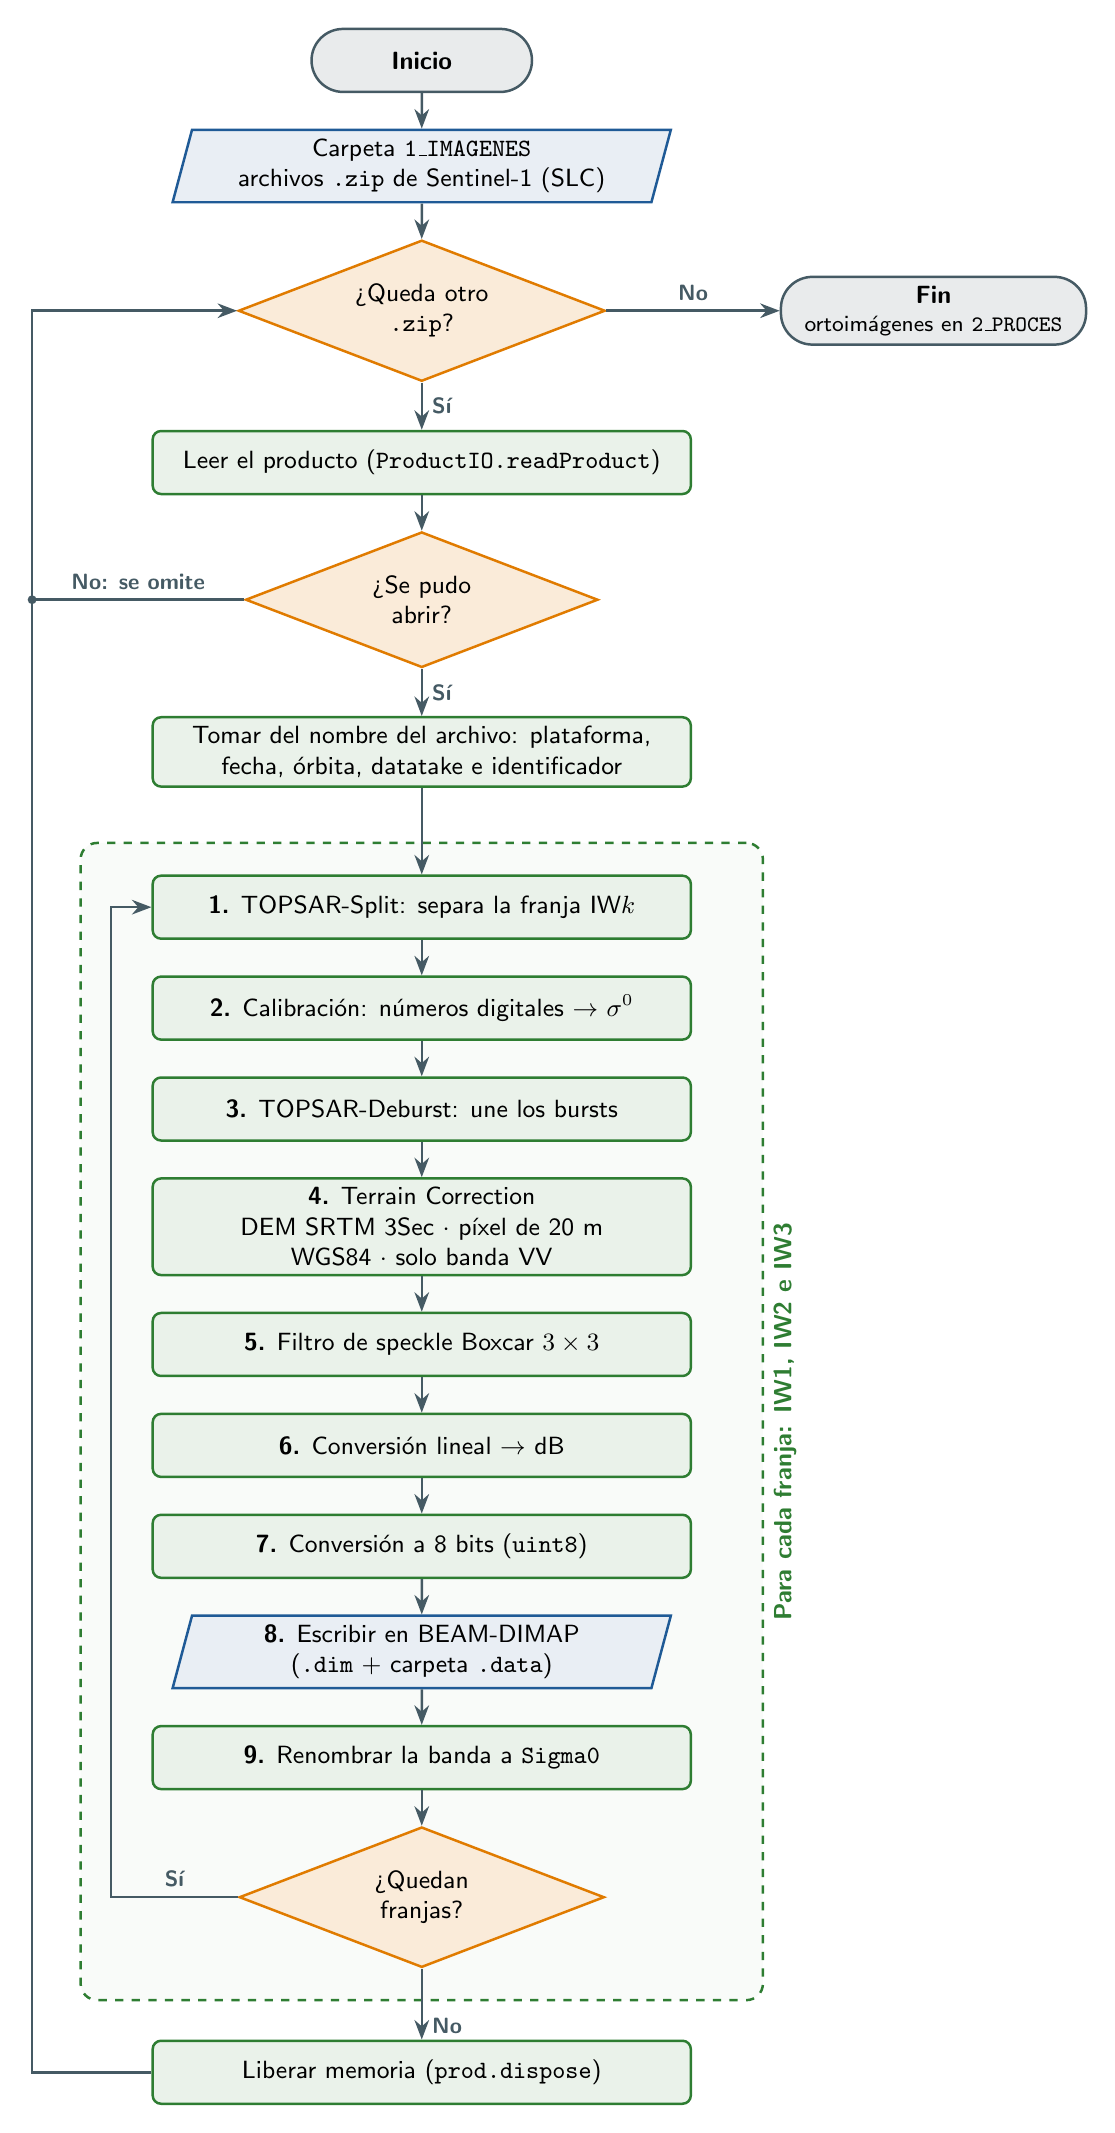
\begin{tikzpicture}[
  >=Stealth,
  node distance=4.5mm,
  proc/.style={rectangle, rounded corners=3pt, draw=verde, line width=0.9pt,
               fill=verde!10, text width=6.6cm, align=flush center,
               minimum height=8mm, font=\small},
  datos/.style={trapezium, trapezium left angle=75, trapezium right angle=105,
                trapezium stretches=true, draw=azul, line width=0.9pt,
                fill=azul!10, text width=5.6cm, align=flush center,
                minimum height=9mm, font=\small},
  dec/.style={diamond, aspect=2.6, draw=naranja, line width=0.9pt,
              fill=naranja!15, text width=2.9cm, align=flush center,
              inner sep=0pt, font=\small},
  term/.style={rectangle, rounded corners=4mm, draw=gris, line width=0.9pt,
               fill=gris!12, minimum width=2.8cm, minimum height=8mm,
               inner xsep=3mm, align=flush center, font=\small\bfseries},
  flecha/.style={->, line width=0.9pt, draw=gris},
  etq/.style={font=\footnotesize\bfseries, text=gris}
]

% ---------- flujo principal ----------
\node[term] (ini) {Inicio};
\node[datos, below=of ini] (in) {Carpeta \texttt{1\_IMAGENES}\\ archivos \texttt{.zip} de Sentinel-1 (SLC)};
\node[dec, below=of in] (hay) {¿Queda otro\\ \texttt{.zip}?};
\node[proc, below=6mm of hay] (leer) {Leer el producto (\texttt{ProductIO.readProduct})};
\node[dec, below=of leer] (ok) {¿Se pudo\\ abrir?};
\node[proc, below=6mm of ok] (nom) {Tomar del nombre del archivo: plataforma,\\ fecha, órbita, datatake e identificador};

% ---------- ciclo por franja ----------
\node[proc, below=11mm of nom] (s1) {\textbf{1.} TOPSAR-Split: separa la franja IW$k$};
\node[proc, below=of s1] (s2) {\textbf{2.} Calibración: números digitales $\rightarrow$ $\sigma^0$};
\node[proc, below=of s2] (s3) {\textbf{3.} TOPSAR-Deburst: une los bursts};
\node[proc, below=of s3] (s4) {\textbf{4.} Terrain Correction\\
  DEM SRTM 3Sec $\cdot$ píxel de 20~m\\ WGS84 $\cdot$ solo banda VV};
\node[proc, below=of s4] (s5) {\textbf{5.} Filtro de speckle Boxcar $3\times3$};
\node[proc, below=of s5] (s6) {\textbf{6.} Conversión lineal $\rightarrow$ dB};
\node[proc, below=of s6] (s7) {\textbf{7.} Conversión a 8 bits (\texttt{uint8})};
\node[datos, below=of s7] (s8) {\textbf{8.} Escribir en BEAM-DIMAP\\ (\texttt{.dim} + carpeta \texttt{.data})};
\node[proc, below=of s8] (s9) {\textbf{9.} Renombrar la banda a \texttt{Sigma0}};
\node[dec, below=of s9] (mas) {¿Quedan\\ franjas?};

\node[proc, below=9mm of mas] (disp) {Liberar memoria (\texttt{prod.dispose})};

\node[term, right=22mm of hay] (fin) {Fin\\[-1pt]\footnotesize\mdseries ortoimágenes en \texttt{2\_PROCES}};

% caja del ciclo
\begin{scope}[on background layer]
  \node[draw=verde, dashed, line width=0.9pt, rounded corners=6pt,
        fill=verde!3, fit=(s1)(mas), inner xsep=9mm, inner ysep=4mm] (caja) {};
\end{scope}
\node[font=\small\bfseries, text=verde, rotate=90, anchor=north]
  at (caja.east) {Para cada franja: IW1, IW2 e IW3};

% coordenadas guía para los retornos
\coordinate (L) at ($(caja.west)+(-6mm,0)$);
\coordinate (M) at ($(caja.west)+(4mm,0)$);

% ---------- flechas ----------
\draw[flecha] (ini) -- (in);
\draw[flecha] (in) -- (hay);
\draw[flecha] (hay) -- node[etq, right]{Sí} (leer);
\draw[flecha] (hay.east) -- node[etq, above]{No} (fin.west);
\draw[flecha] (leer) -- (ok);
\draw[flecha] (ok) -- node[etq, right]{Sí} (nom);
\draw[flecha] (nom) -- (s1);
\foreach \a/\b in {s1/s2, s2/s3, s3/s4, s4/s5, s5/s6, s6/s7, s7/s8, s8/s9, s9/mas}
  \draw[flecha] (\a) -- (\b);
\draw[flecha] (mas) -- node[etq, right, pos=0.8]{No} (disp);

% retorno del ciclo de franjas
\draw[flecha] (mas.west) -- node[etq, above]{Sí} (M |- mas.west) |- (s1.west);

% retorno al siguiente .zip
\draw[flecha] (disp.west) -| (L |- hay.west) -- (hay.west);
\draw[line width=0.9pt, draw=gris] (ok.west) -- node[etq, above]{No: se omite} (L |- ok.west);
\fill[gris] (L |- ok.west) circle (1.6pt);

\end{tikzpicture}
\end{document}
